\documentclass[../main/main.tex]{subfiles}
\graphicspath{{./figures/}}

\makeatletter
\renewcommand{\@chapapp}{Travaux pratiques -- TP}
\makeatother

\toggletrue{student}
\HideSolutionstrue

\begin{document}
\setcounter{chapter}{2}

\chapter{Images \`a l'infini~: utilisation de la lunette autocollimatrice}

\ifstudent{
	\begin{prgm}
		\begin{tcb}*(ror)"how"{Savoir-faire}
			\begin{itemize}[label=$\diamond$, leftmargin=10pt]
				\item Mesure de longueurs sur un banc d'optique.
				\item Mettre en œuvre une mesure de longueur par déplacement du viseur
				      entre deux positions.
				\item Utiliser un viseur à frontale fixe, une lunette auto-collimatrice.
				\item Utiliser des vis micrométriques et un réticule pour
				      tirer parti de la précision affichée de l'appareil utilisé.
			\end{itemize}
		\end{tcb}
	\end{prgm}
	\vspace{-10pt}
	\section{Objectifs}
	\begin{itemize}
		\item Utiliser une lunette autocollimatrice pour~:
		      \begin{enumerate}
			      \item Reconnaître un faisceau parallèle~;
			      \item Utiliser un faisceau parallèle~;
		      \end{enumerate}
		\item Continuer à se familiariser avec un viseur à frontale fixe~;
		\item Réaliser des régressions linéaires.
	\end{itemize}
}

\section{S'approprier}

\subsection{Principe de la lunette autocollimatrice}

\noindent
\begin{minipage}[c]{.4\linewidth}
	La lunette autocollimatrice permet de réaliser un faisceau de lumière
	parallèle. Elle est constituée d'un objectif, d'un réticule $R$ et d'un
	oculaire. Entre l'oculaire et le réticule est disposée une lame
	semi-réfléchissante, inclinée à $\ang{45;;}$ par rapport à l'axe optique du
	dispositif et éclairée par une petite ampoule (éclairage auxiliaire).
\end{minipage}
\hfill
\begin{minipage}[c]{.55\linewidth}
	~
	\begin{center}
		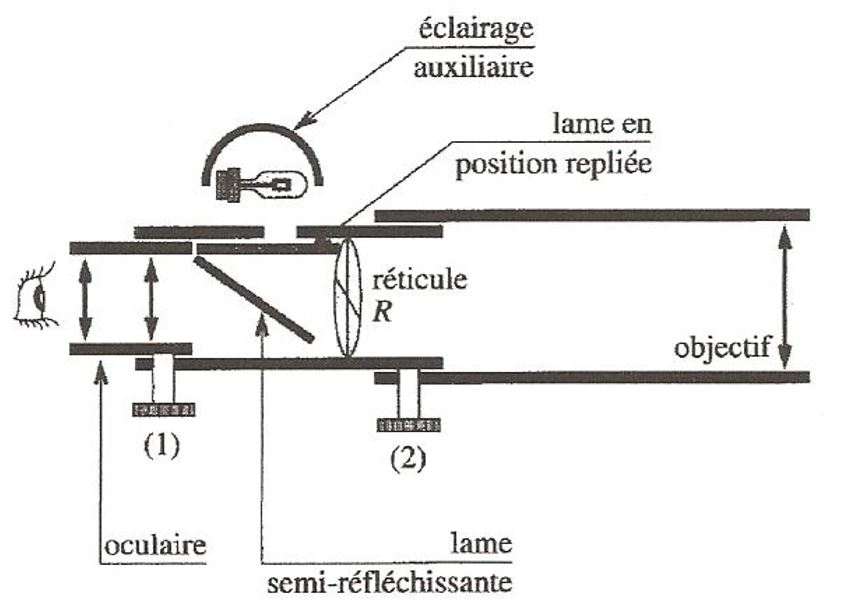
\includegraphics[width=\linewidth]{lunette_auto}
	\end{center}
\end{minipage}

\subsection{Théorème des vergences}

\ifstudent{
	Considérons deux lentilles minces $\Lc_1$ et $\Lc_2$ de centres optiques
	respectifs O$_1$ et O$_2$ et de distances focales images respectives $f'_1$ et
	$f'_2$. On suppose que ces deux lentilles sont accolées si bien que leurs
	centres optiques sont confondus~: $\rm O_1 \equiv O_2 \equiv O$.
}

\begin{enumerate}[label=\clenumi]
	\item \switch{
	      Redémontrez le théorème des vergences.
	      }{
	      Soit un objet $\ABr$ conjugué à son image $\rm A_2B_2$ par le doublet de
	      lentilles. Par ailleurs, on introduit $\ABb$ l'image intermédiaire. Nous
	      pouvons alors écrire la relation de conjugaison de Descartes pour
	      chacune des lentilles~:
	      \[
		      \frac{1}{\obar{\rm OA_1}}-\frac{1}{\obar{\rm OA}} =
		      \frac{1}{f'_1}
		      \qqet
		      \frac{1}{\obar{\rm OA_2}}-\frac{1}{\obar{\rm OA_1}} =
		      \frac{1}{f'_2}
	      \]
	      Sommons terme à terme ces deux relations. Il vient alors~:
	      \[
		      \frac{1}{\obar{\rm OA_2}}-\frac{1}{\obar{\rm OA}} =
		      \frac{1}{f'_1}+\frac{1}{f'_2}
	      \]
	      Si bien que tout se passe comme si le système optique était équivalent à une
	      unique lentille mince de distance focale image $f'_{\rm eq}$ tel que~:
	      \[
		      \frac{1}{f'_{\rm eq}}= \frac{1}{f'_1}+\frac{1}{f'_2}
	      \]
	      \leftencadre{Soit encore, en terme de vergences~:
	      }{
		      $V_{\rm eq} = V_1+V_2$}
	      }
\end{enumerate}

\subsection{Réglage de l'oculaire}

Même principe que pour régler le viseur~:

\begin{tcb}(expe){Réglage de l'oculaire}
	\begin{enumerate}
		\item Allumer la lampe latérale de la lunette qui éclaire le réticule.
		      \textbf{Attention} elle doit être alimentée en $\SI{6}{V}$ alternatif.
		      Sinon vous risquez de l'endommager.
		\item Régler l'oculaire à votre vue~: mettre au point le réticule en
		      agissant sur l'œilleton de l'oculaire grâce à la vis (1). Ce réglage est
		      personnel et nécessaire avant toute manipulation. La lunette est réglée
		      quand on voit les deux fils croisés nets.
	\end{enumerate}
\end{tcb}

\subsection{Réglage de la lunette sur l'infini}

On effectue ce réglage pour obtenir un faisceau de lumière parallèle. Il se fait
à l'aide d'un miroir plan.

\begin{tcb}(expe){Réglage sur l'infini}
	\begin{enumerate}
		\item Placer la lame semi-réfléchissante interne de telle façon que la
		      lumière sorte de l'objectif (loquet argenté). Pour cela, vérifier qu'un
		      faisceau lumineux est visible en mettant votre main à la sortie de la
		      lunette.
		\item Placer sur l'objectif (immédiatement après la lunette) le petit miroir
		      plan.
		\item Observer l'image en retour du réticule: déplacer l'ensemble oculaire
		      par rapport à l'objectif de façon à ce que cette image en retour soit
		      aussi nette que l'objet, en agissant sur la bague moletée (2) de la
		      lunette.
	\end{enumerate}
\end{tcb}

On vient alors de réaliser un réglage par autocollimation. Ainsi, on s'assure
que \textbf{le réticule est au foyer objet de l'objectif}. La lunette peut ainsi
être utilisée~:
\begin{itemize}
	\item Pour reconnaître un faisceau parallèle (1er montage),
	\item Comme source de faisceau parallèle (2ème montage).
\end{itemize}

\section{Réaliser et valider}

Activité \texttt{Capytale}
disponible\ftn{\url{https://capytale2.ac-paris.fr/web/c/89bb-1898302}}.

\subsection{Détermination d'une distance focale}

L'objectif de cette partie est de déterminer la distance focale d'une lentille
expérimentalement (focométrie) par reconnaissance d'une faisceau parallèle en
utilisant la lunette autocollimatrice.

\subsubsection{Montage}

\begin{center}
	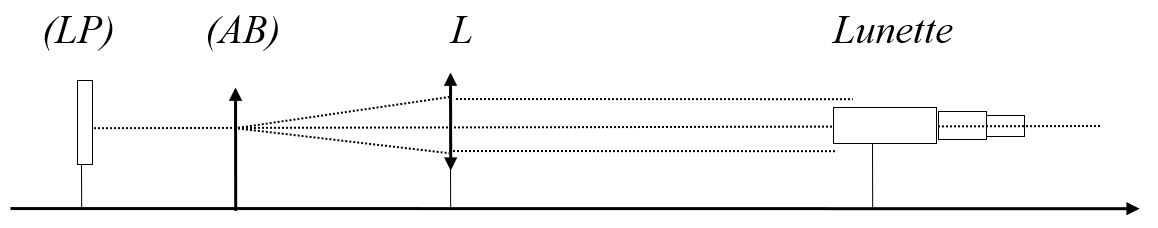
\includegraphics[width=0.8\textwidth]{montage_foc_lunette}
\end{center}

\begin{tcb}(expe){}
	\begin{enumerate}
		\item Prendre comme objet $\ABr$, la plaque constituée des lettres F sur
		      support translucide et prendre une lentille de distance focale
		      $\SI{10}{cm}$ ou $\SI{20}{cm}$. Éclairer l'objet $\ABr$ avec la lampe
		      spectrale $(LP)$. Cette lampe doit être allumée une dizaine de minutes
		      avant l'expérience pour chauffer. Interposer un dépoli devant la lampe
		      pour limiter la luminosité et protéger vos yeux.
		\item Réaliser le montage ci-dessus, en mettant la lunette à droite de la
		      lentille, sa place a peu d'importance. La lame semi-réflechissante à
		      l'intérieur de la lunette doit être rétractée.
		\item Déplacer la lentille pour voir dans la lunette autocollimatrice
		      l'image $\ABpr$ de $\ABr$ nette sur le réticule~: $\ABpr$ est alors à
		      l'infini donc $\ABr$ est dans le plan focal objet de la lentille.
	\end{enumerate}
\end{tcb}

Vérifier que la position de la lunette n'a pas d'importance en la déplaçant sur
le banc optique, ce qui montre l'existence d'un faisceau de lumière parallèle.

\subsubsection{Mesure de la distance focale}

\begin{enumerate}[label=\sqenumi]
	\item Estimer alors la distance focale $f'$ de la lentille, ainsi que son
	      incertitude.
	\item \switch{
		      Calculer l'écart normalisé et conclure.
	      }{
		      On peut alors estimer la distance focale $f'$ de la lentille en
		      mesurant grâce au réglet fixé sur le banc optique la distance entre
		      l'objet et la lentille. Si vous constatez un désaccord trop grand
		      entre la valeur prévue et la valeur obtenue, essayez de trouver la
		      cause de l'erreur systématique qui est créée par le montage. Ce
		      montage est moins précis que celui vu au TP précédent pour déterminer
		      la distance focale d'une lentille, mais il est également bien plus
		      rapide~!
	      }
\end{enumerate}

\subsection{Vérification du théorème des vergences}

\subsubsection{Montage}

\begin{center}
	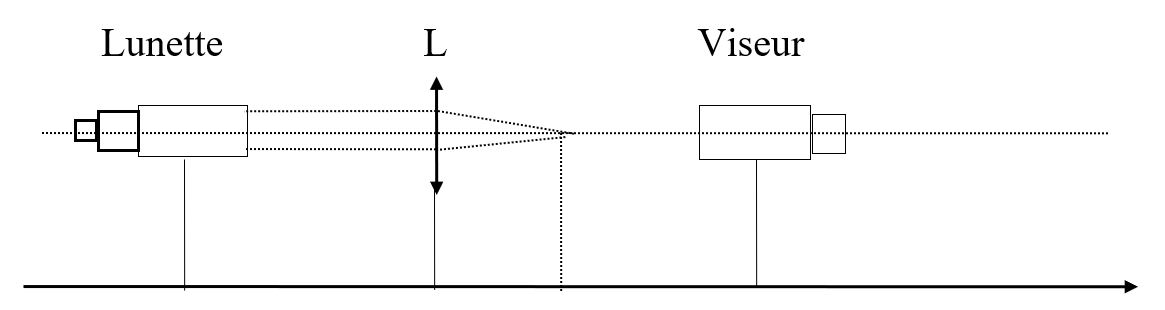
\includegraphics[width=0.8\textwidth]{montage_verg_lunette}
\end{center}

\begin{tcb}(expe){}
	\begin{enumerate}
		\item Éteindre la lanterne utilisée dans le montage précédent. La source
		      secondaire de la lunette autocollimatrice est maintenant la source de
		      lumière. La mettre à gauche sur le banc d'optique. Elle doit toujours
		      être réglée sur l'infini. Interposer une lentille convergente entre la
		      lunette et un viseur à frontale fixe. Soignez vos alignements.

		\item Repérer la position du viseur à frontale fixe permettant d'observer
		      la face de sortie de la lentille (mettre un petit morceau de papier sur
		      cette face ou la mine de votre crayon). On notera cette position $x_v$.

		\item Ensuite, viser l'image du réticule avec le viseur et relever la
		      position $x_{R}$ du viseur à frontale fixe correspondante sur le banc
		      optique. Vous chercherez cette position en éloignant le viseur d'environ
		      la distance focale de la lentille par rapport à la position $x_v$
		      précédemment obtenue.
	\end{enumerate}
\end{tcb}

\begin{enumerate}[label=\sqenumi, start=3]
	\item Faire la manipulation avec les différentes lentilles convergentes
	      dont vous disposez, en notant l'incertitude et en calculant les écarts
	      normalisés. Sur vos compte-rendus, vous ordonnerez vos résultats dans un
	      tableau sous la forme suivante~:
\end{enumerate}

\begin{table}[htbp]
	\centering
	\caption{Relevés de distances focales}
	\begin{tabular}{cccccc}
		\toprule
		Numéro   & $f_{\rm theo} (\si{cm})$ & $x_v (\si{cm})$ & $x_R (\si{cm})$ & $f_{\rm exp} (\si{cm})$ & $E_N$
		\\
		0        & …                        & … $\pm $ …      & … $\pm $ …      & … $\pm $ …              & …
		\\
		1        & …                        & … $\pm $ …      & … $\pm $ …      & … $\pm $ …              & …
		\\
		2        & …                        & … $\pm $ …      & … $\pm $ …      & … $\pm $ …              & …
		\\
		3        & …                        & … $\pm $ …      & … $\pm $ …      & … $\pm $ …              & …
		\\
		4        & …                        & … $\pm $ …      & … $\pm $ …      & … $\pm $ …              & …
		\\
		$\vdots$ & $\vdots$                 & $\vdots$        & $\vdots$        & $\vdots$
		         & $\vdots$
		\\
		\bottomrule
	\end{tabular}
\end{table}

\subsubsection{Validation du théorème des vergences}

\begin{tcb}(expe){}
	\begin{enumerate}
		\item Prendre la lentille convergente de distance focale connue $+8\delta$.

		\item Associer à cette lentille (en les disposant accolées à la première),
		      une par une, les autres lentilles dont vous disposez (convergentes ou
		      divergentes).
	\end{enumerate}
\end{tcb}

\begin{enumerate}[label=\sqenumi, start=4]
	\item En utilisant la méthode précédente, mesurer la distance focale totale
	      $f'_{\rm tot, exp}$ pour chaque association de lentilles, et en déduire
	      la vergence expérimentale de l'ensemble. Réaliser au moins cinq
	      associations différentes. Sur vos compte-rendus, vous ordonnerez vos
	      résultats dans un tableau sous la forme suivante~:
	      \begin{table}[htbp]
		      \centering
		      \caption{Relevés de vergences}
		      \begin{tabular}{ccccccccc}
			      \toprule
			      Numéro   & $V_1 (\delta)$ & $V_2(\delta)$ & $V_{\rm tot, theo}(\delta)$ & $x_v (\si{cm})$ & $x_R (\si{cm})$ & $f'_{\rm tot, exp} (\si{cm})$ & $V_{\rm tot, exp} (\delta)$ & $E_N$
			      \\
			      0        & $8 $           & …             & …                           & … $\pm $ …      & … $\pm $ …      & … $\pm $ …                    & … $\pm $ …                  & …
			      \\
			      1        & $8 $           & …             & …                           & … $\pm $ …      & … $\pm $ …      & … $\pm $ …                    & … $\pm $ …                  & …
			      \\
			      2        & $8 $           & …             & …                           & … $\pm $ …      & … $\pm $ …      & … $\pm $ …                    & … $\pm $ …                  & …
			      \\
			      3        & $8 $           & …             & …                           & … $\pm $ …      & … $\pm $ …      & … $\pm $ …                    & … $\pm $ …                  & …
			      \\
			      $\vdots$ & $\vdots$       & $\vdots$      & $\vdots$                    & $\vdots$        & $\vdots$        & $\vdots$                      & $\vdots$                    & $\vdots$
			      \\
			      \bottomrule
		      \end{tabular}
	      \end{table}

	      \begin{tcb}(impo){Attention}
		      \begin{enumerate}[label=\arabic*)]
			      \item $x_v$ doit correspondre à la visée du milieu des deux
			            lentilles. On placer un bout de papier placé \textit{entre
				            les deux lentilles} pour cela.
			      \item L'incertitude d'un inverse n'est pas la même incertitude…
		      \end{enumerate}
	      \end{tcb}
\end{enumerate}

\begin{enumerate}[label=\clenumi, start=2]
	\item Quelle régression linéaire doit-on effectuer~?
\end{enumerate}

\begin{enumerate}[label=\sqenumi, start=5]
	\item Réaliser ensuite une régression linéaire \textbf{à la calculatrice} de
	      la vergence totale expérimentale en fonction de la vergence ajoutée pour
	      chacune des lentilles. Relever les valeurs de $a$ (coefficient
	      directeur), $b$ (ordonnée à l'origine) et $r$ (coefficient de
	      corrélation) données par la calculatrice.
	\item Ces valeurs de $a$ et $b$ vous semblent-elles cohérentes~? Justifier.
	\item Reprendre les deux dernières questions avec l'activité
	      \texttt{Capytale}.
\end{enumerate}

\end{document}
